\section{\textsf{Simulation}} 
    The simulation was conducted using CST (Computer Simulation Technology)
    software to implement a configuration inspired by the design presented 
    in \cite{zhang_design_2023}. This section outlines the steps taken to 
    model the structure, the assumptions made, and the results obtained from
    the simulation.

    \subsection{\textsf{CST Implementation}} 
        The vertical layout in CST consists of a three-layer structure:
        \begin{itemize}
        \item \textbf{Dielectric Substrate}:  This layer serves as the 
            base for the structure.
        \item \textbf{Air Gap}: Positioned above the dielectric substrate,
            this layer introduces an air gap to influence the electromagnetic 
            properties.
        \item \textbf{Metal Backplate}: The top layer, made of copper, 
            acts as a reflective surface.
        \end{itemize}

        The dielectric substrate also includes a metallic component, which
        is made of the same material as the metal backplate—copper, with
        a conductivity of (5.96 \mu $10^7$ S/m).

        Initially, the FR-4 substrate is placed without the metal 
        resonance layer. The other two layers are positioned below $Z=0$. 
        When viewed from the orthographic side, the layout appears as shown
        in Figure \ref{img:layout}.
        \begin{figure}[h]
            \centering
            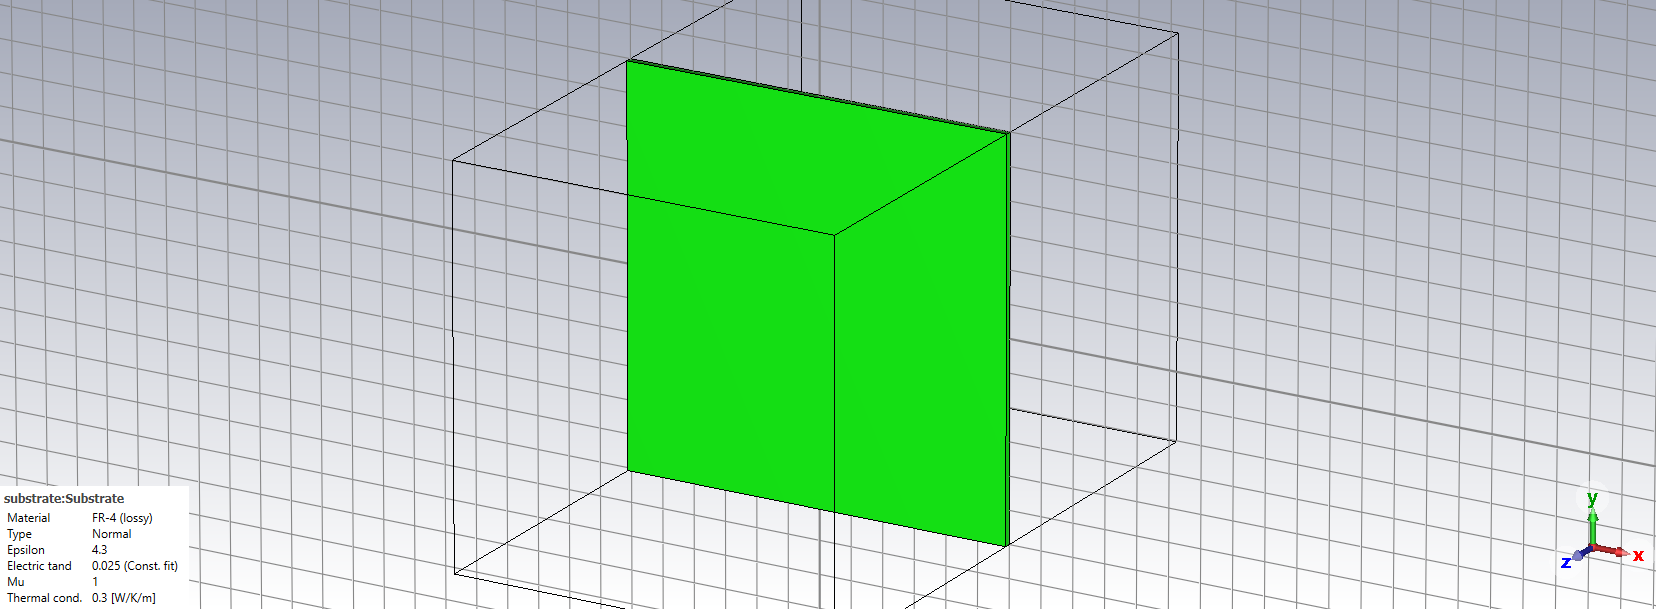
\includegraphics[width=0.4\textwidth]{substrate.png}\hfil
            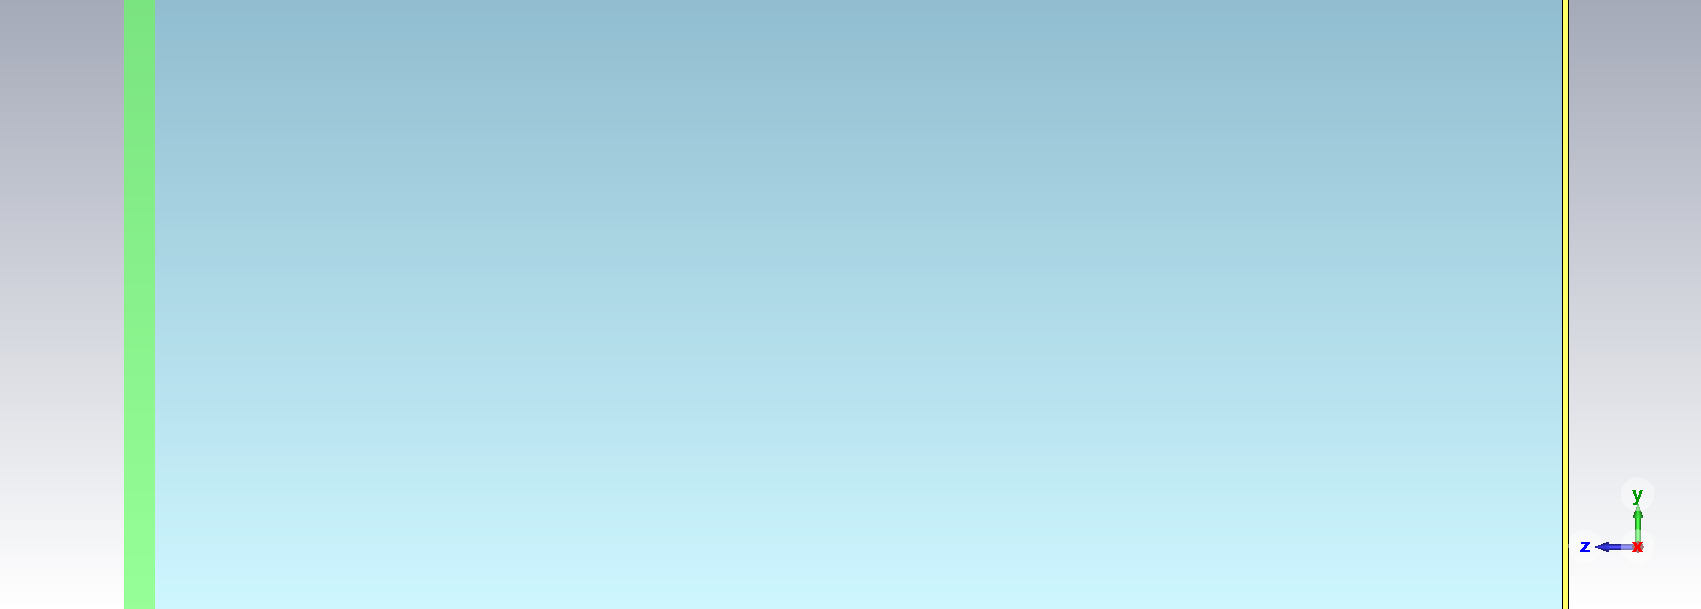
\includegraphics[width=0.4\textwidth]{verticaLayout.png}
            \caption{Basic Vertical Layout}
            \label{img:layout}
        \end{figure}

        Next, a ring resonator is added on top of the dielectric substrate. 
        The ring is made of the same material and thickness as the backplate, 
        as illustrated in Figure \ref{img:ring}.
        \begin{figure}[h]
            \centering
            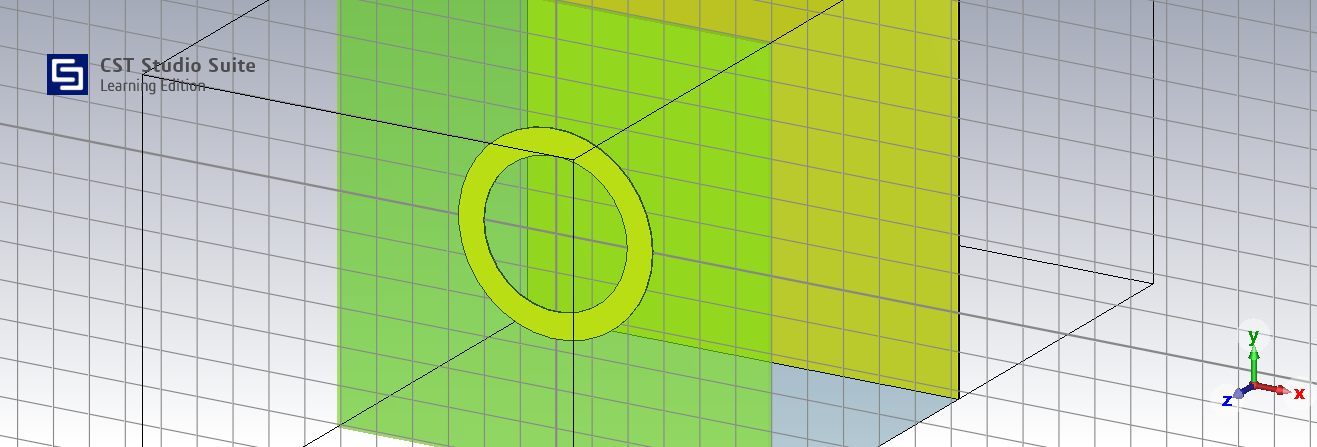
\includegraphics[width=0.6\textwidth]{ring.png}
            \caption{Ring Resonator}
            \label{img:ring}
        \end{figure}

        An important assumption in this design is that both the body and the 
        tip of the arrow have a width of $\alpha=0.5 mm$. To accurately place
        the curve points defining the arrow, a system of equations must be 
        solved to determine the Cartesian coordinates of the arrow's base points. 
        These points lie on the arc of the ring and are equidistant from the curve 
        $y=x$. The following MATLAB code snippet demonstrates the solution to this 
        system:
        \begin{lstlisting}[frame=single, numbers=left, style=Matlab-Pyglike]
            syms x1 x2

            eq1 = 2*(x1 - x2)^2 == .5^2; eq2 = sqrt(x2^2 + x1^2) == 2.7;

            sol = solve([eq1, eq2], [x1 x2]); disp([sol.x1 sol.x2]);  
        \end{lstlisting}
        
        This system simplifies to the equations shown in Equation \ref{eq:xysys}.
        \begin{equation}
            \label{eq:xysys}
            \displaystyle \begin{array}{l} 
                \left(\begin{array}{cc} 
                    \sigma_3 -\frac{2916\,\sigma_1 }{1433} & -\sigma_1 \\
                    \sigma_4 -\frac{2916\,\sigma_2 }{1433} & -\sigma_2 \\
                    \frac{2916\,\sigma_1 }{1433}-\sigma_3  & \sigma_1 \\
                    \frac{2916\,\sigma_2 }{1433}-\sigma_4  & \sigma_2  
                \end{array}\right)\\
                \mathrm{}\\
                \textrm{where}\\
                \mathrm{}\\
                \;\;\sigma_1 =\sqrt{\frac{729}{200}-\frac{7\,\sqrt{59}}{80}}\\
                \mathrm{}\\
                \;\;\sigma_2 =\sqrt{\frac{7\,\sqrt{59}}{80}+\frac{729}{200}}\\
                \mathrm{}\\
                \;\;\sigma_3 =\frac{400\,{{\left(\frac{729}{200}-\frac{7\,\sqrt{59}}{80}\right)}}^{3/2} }{1433}\\
                \mathrm{}\\
                \;\;\sigma_4 =\frac{400\,{{\left(\frac{7\,\sqrt{59}}{80}+\frac{729}{200}\right)}}^{3/2} }{1433}
            \end{array}
        \end{equation}

        The arrow is then mirrored across the X, Y, and XY planes to cover all
        four sides of the cell. The face is covered with copper, and a height of 
        $d=0.035 mm$ is assigned, as shown in Figure \ref{img:mirrorAndCover}. 
        This step is crucial because all other layers were initially positioned 
        below $Z=0$.
        \begin{figure}[h]
            \centering
            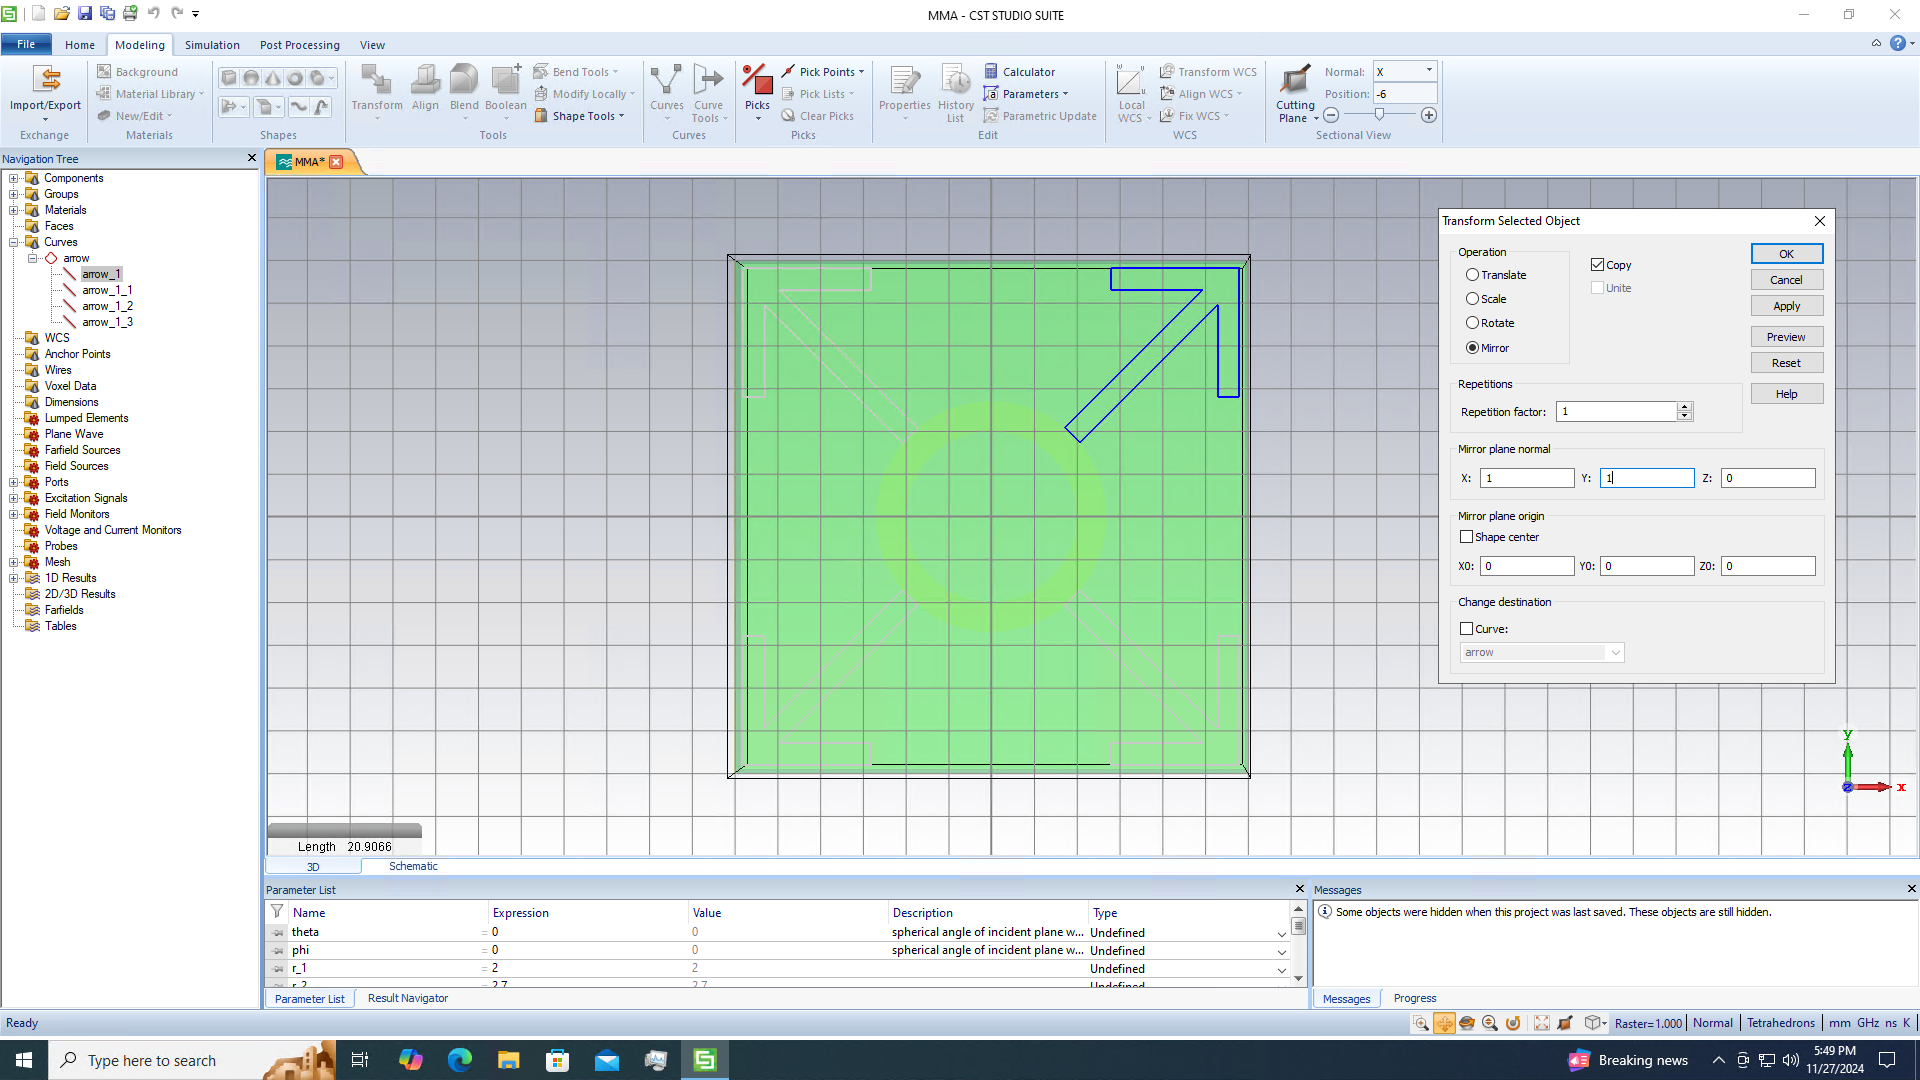
\includegraphics[width=.4\textwidth]{mirroredArrows.png}\hfil
            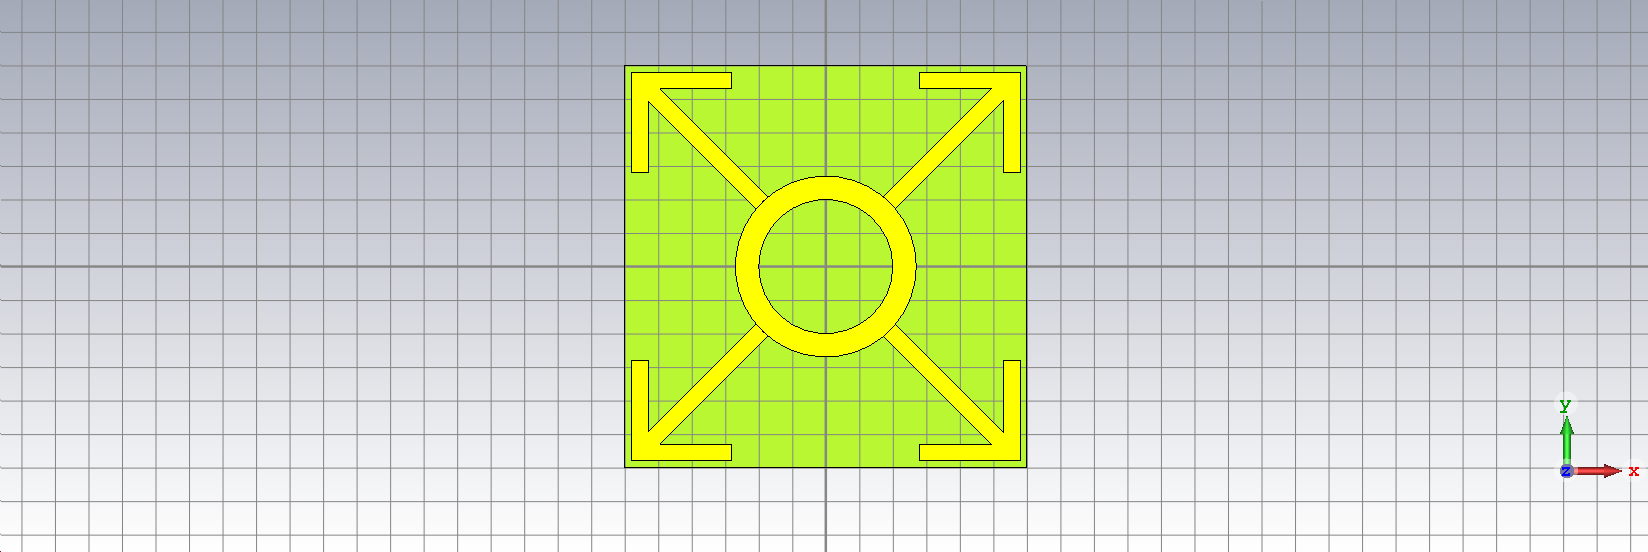
\includegraphics[width=.4\textwidth]{RingAndArrows.png}
            \caption{Mirroring Arrow and Cover}
            \label{img:mirrorAndCover}
        \end{figure}

        A series of cuts (boolean subtractions) are made in the resonance layer
        to add resistors between the copper faces near the arrows, as depicted 
        in Figure \ref{img:arrowCuts}.
        \begin{figure}[h]
            \centering
            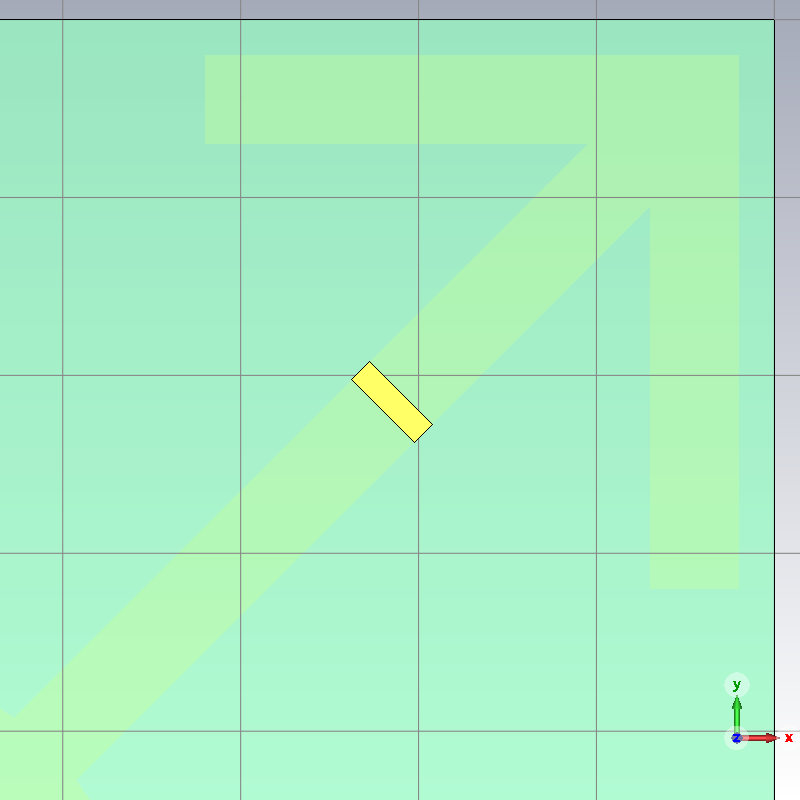
\includegraphics[width=.4\textwidth]{subtract.png}\hfil
            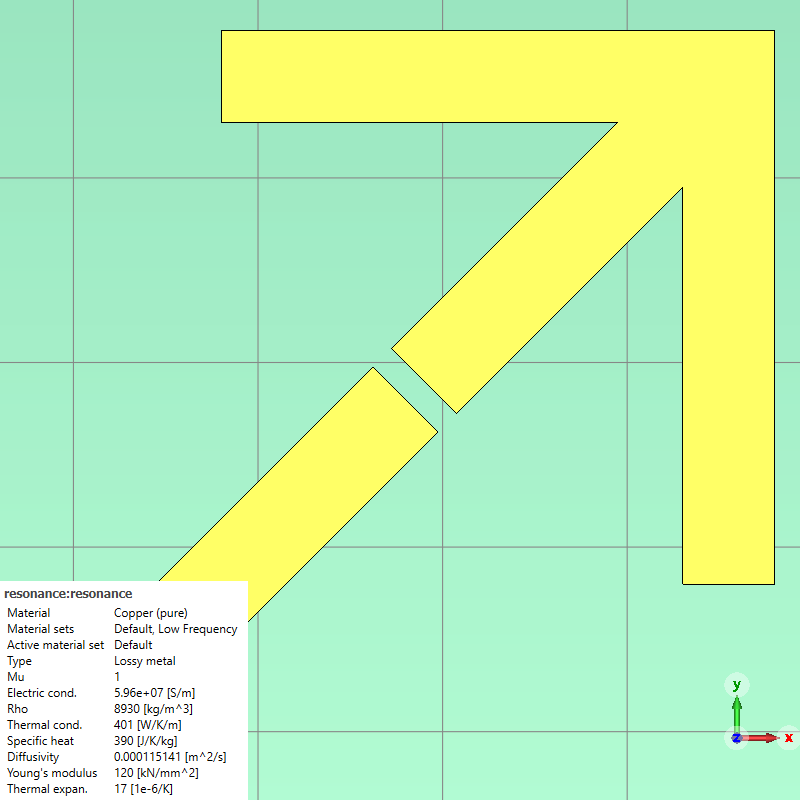
\includegraphics[width=.4\textwidth]{subtracted.png}
            \caption{Cuts Near the Arrows}
            \label{img:arrowCuts}
        \end{figure}

        Similar cuts are made near the ring to ensure uniform width, as shown 
        in Figure \ref{img:ringCuts}.
        \begin{figure}[h]
            \centering
            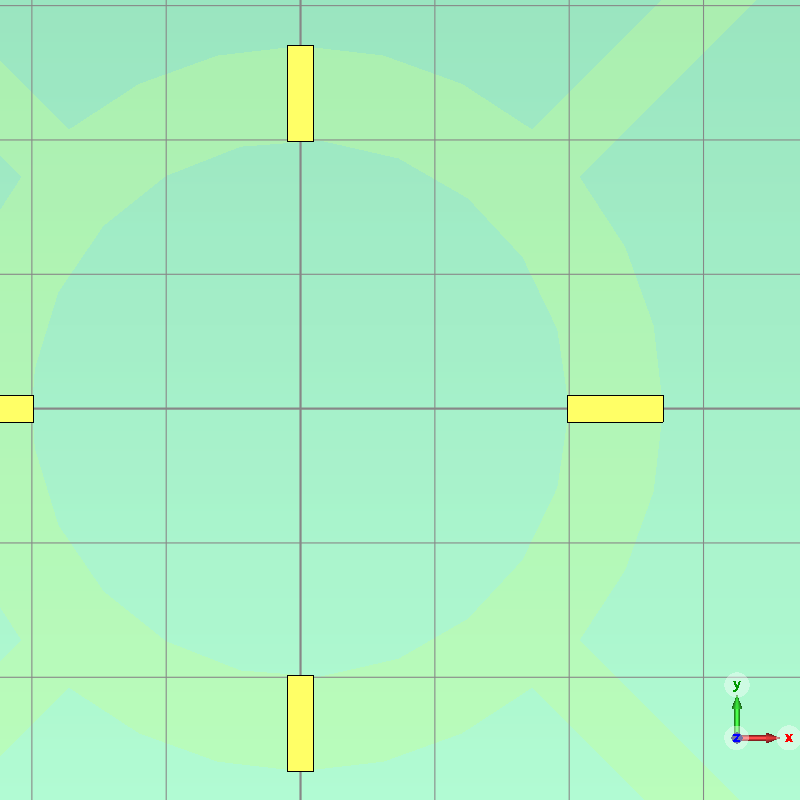
\includegraphics[width=.4\textwidth]{subtractRing.png}\hfil
            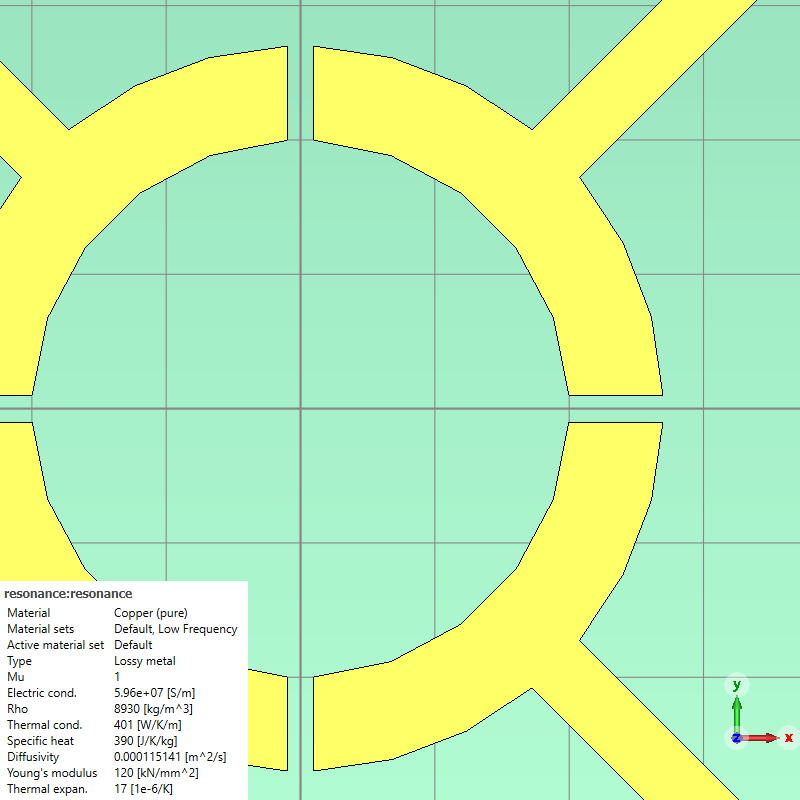
\includegraphics[width=.4\textwidth]{subtractedRing.png}
            \caption{Cuts Near the Ring}
            \label{img:ringCuts}
        \end{figure}

        Resistors are then added, connecting to the center points of the faces
        created by the previous subtractions, as illustrated in Figure 
        \ref{img:resistors}. It is important to note that the performance of 
        the absorber may be reduced in this implementation. Better absorbance 
        might be achieved if the connection height is set to $d=0.035mm$.

        To perform the simulation using the frequency solver in CST, periodic 
        boundaries are set along the XY plane, and free space conditions are 
        applied along the Z axis. The resulting mesh is shown in Figure 
        \ref{img:RingAndArrowMesh}.
        
        \begin{figure}
            \centering
            \begin{subfigure}{0.49\textwidth}
                \centering
                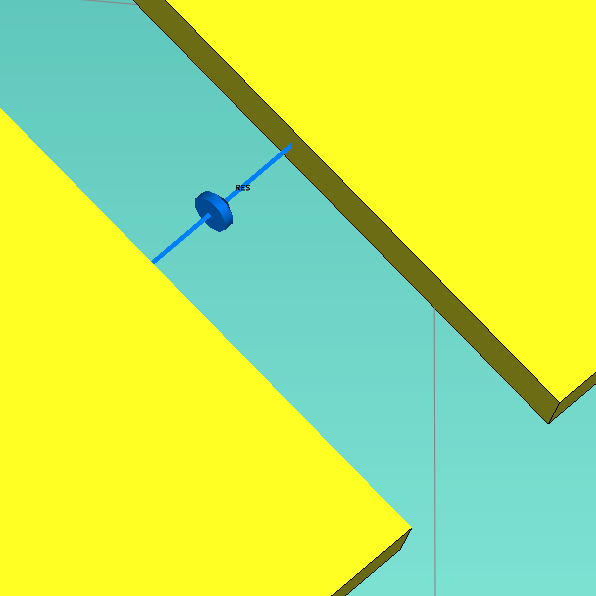
\includegraphics[width=\textwidth]{faceCenterPoint.png}
                \caption{Resistor Placement}
                \label{img:resistors}
            \end{subfigure}
            \hfill
            \begin{subfigure}{0.49\textwidth}
                \centering
                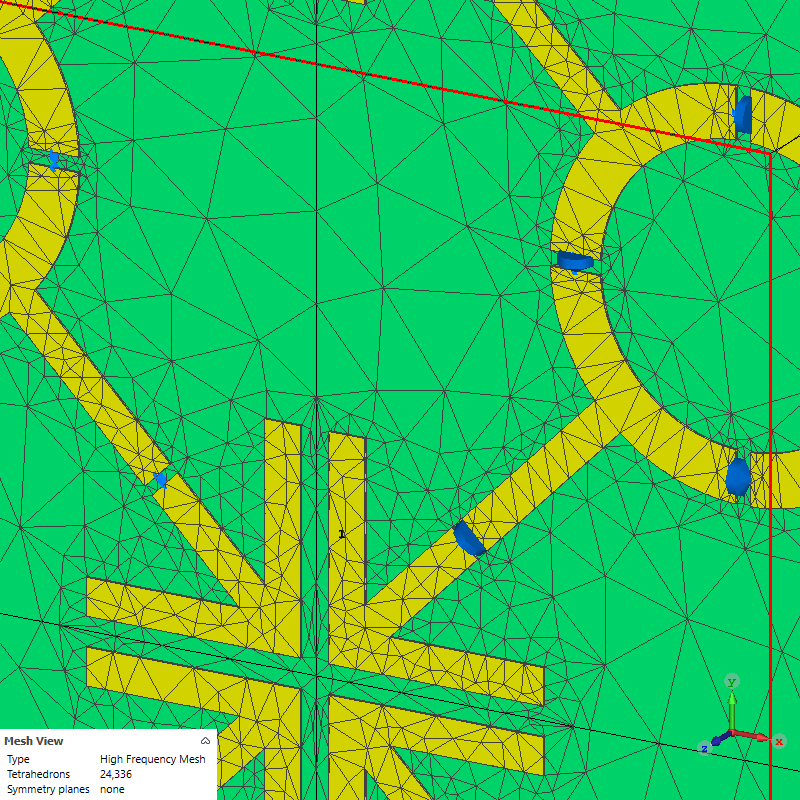
\includegraphics[width=\textwidth]{mesh.png}
                \caption{Ring Mesh for reference}
                \label{img:RingAndArrowMesh}
            \end{subfigure}
            \caption{Mesh around Resistors}
            \label{fig:combined}
        \end{figure}

        The electrical field absorbance is analyzed at different frequencies. 
        Figure \ref{img:E_Zmax1} shows the electrical field for $Z_{max}(1)$
        at frequencies of 2.7 GHz, 7.7 GHz, and 12.7 GHz.
        \begin{figure}[h]
            \centering
            
            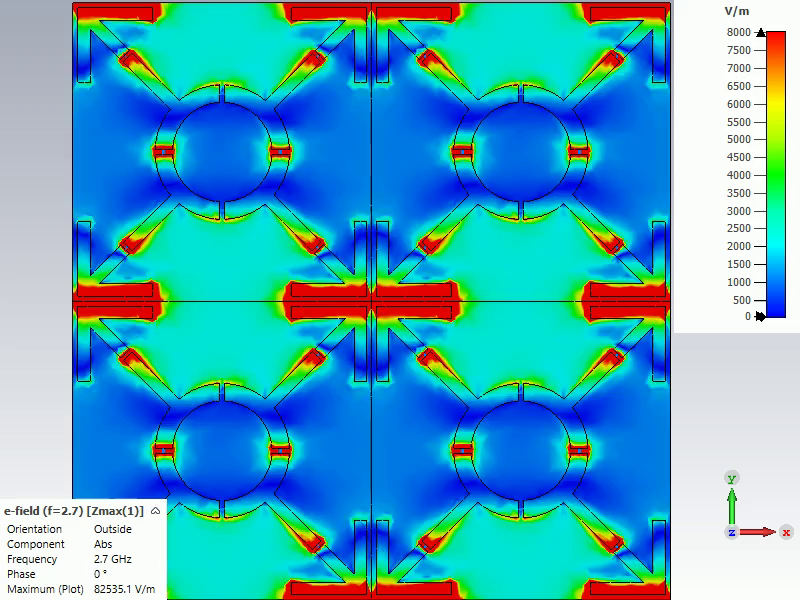
\includegraphics[page=1, width=0.22\textwidth]{E_Zmax1_027e2MHz.png}\hfil
            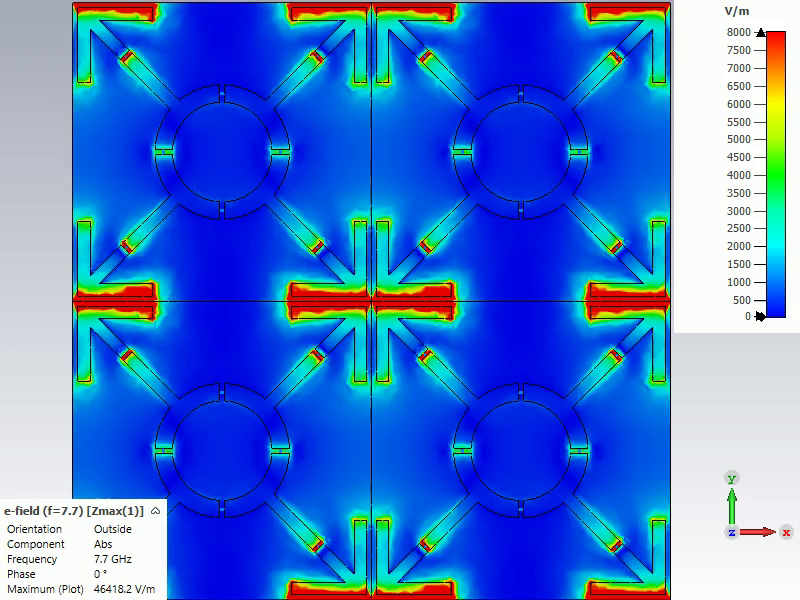
\includegraphics[page=1, width=0.22\textwidth]{E_Zmax1_077e2MHz.png}\hfil
            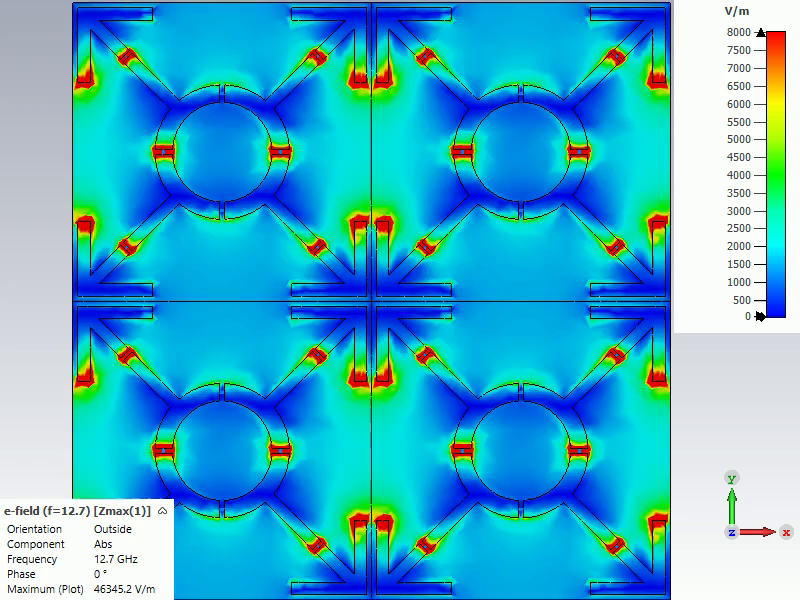
\includegraphics[page=1, width=0.22\textwidth]{E_Zmax1_127e2MHz.png}
            
            \caption{Electrical Field for [2.7, 7.7, 12.7] GHz $Z_{max}(1)$}
            \label{img:E_Zmax1}
        \end{figure}

        Similarly, Figure \ref{img:E_Zmax2} shows the electrical field for $Z_{max}(2)$
        at the same frequencies.
        \begin{figure}[h]
            \centering
            
            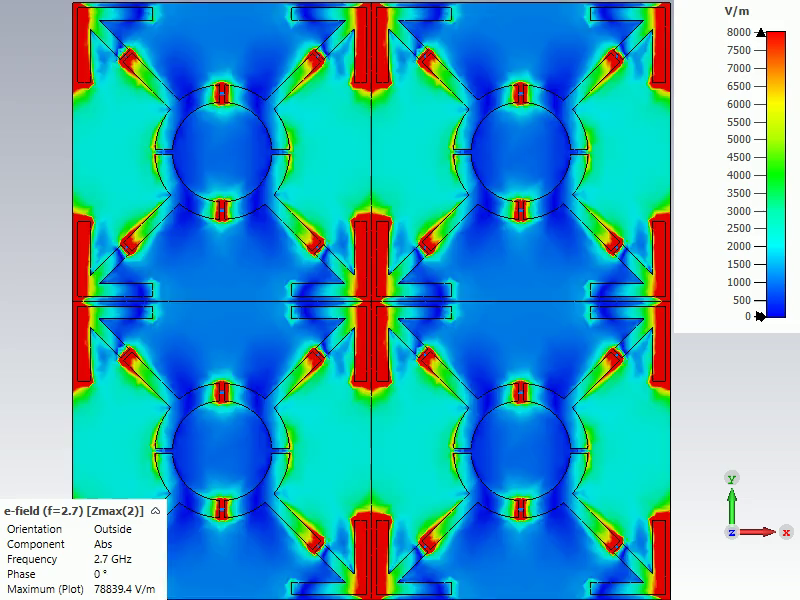
\includegraphics[page=1, width=0.22\textwidth]{E_Zmax2_027e2MHz.png}\hfil
            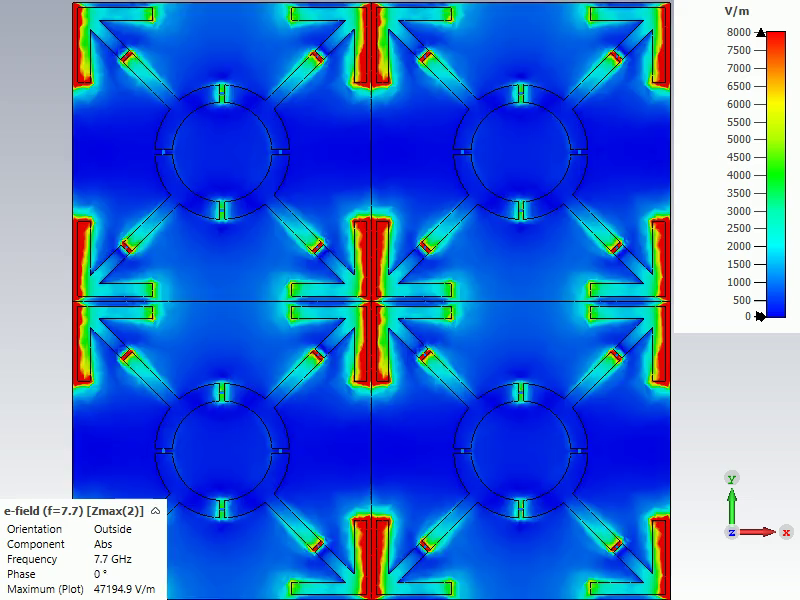
\includegraphics[page=1, width=0.22\textwidth]{E_Zmax2_077e2MHz.png}\hfil
            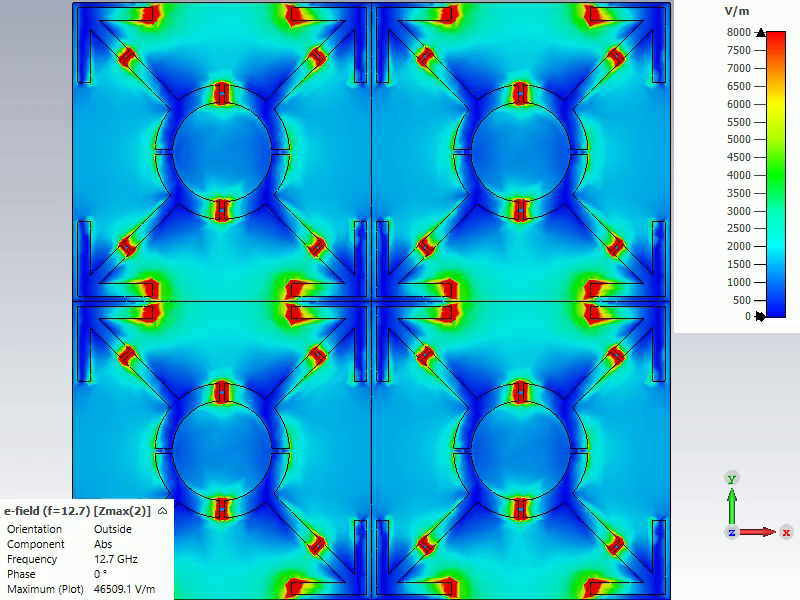
\includegraphics[page=1, width=0.22\textwidth]{E_Zmax2_127e2MHz.png}
            
            \caption{Electrical Field for [2.7, 7.7, 12.7] GHz $Z_{max}(2)$}
            \label{img:E_Zmax2}
        \end{figure}

        Taking a look in the $S_{11}$ of $Z_{max}$ after the simulation as such
        (\ref{plt:S11_Zmax}). The Absorptivity (against the frequency) is an
        essential metric and CST calculates it as shown in (\ref{plt:Absorptivity}).
        For the evaluation of the absorber Absorptivity can be calculated using the
        formula: $ A = 1 - |S_{11}|^2 - |T|^2 $, where T is the transmission
        coefficient and can be calculated using the formula: $T =
        \frac{2Z_0}{Z+Z_0}$. However the $Z$ mentioned needs to be the normalized
        impedance of the absorber so this is where the calculation will start.

        \begin{center}
            \begin{minipage}{.45\textwidth}
                \begin{tikzpicture}
                    \begin{axis}[ 
                        title={\textsf{Reflection Coefficient}},
                        xlabel={Frequency (GHz)}, ylabel={$S_{11}$ (dB)} 
                    ] \addplot table[x=freq, y=s11, col sep=space] {data/s11.txt};
                    \end{axis}
                \end{tikzpicture}
                %\captionof{figure}{\textsf{The $S_{11}$}}
                \label{plt:S11_Zmax}
            \end{minipage}
            \begin{minipage}{.45\textwidth}
                \begin{tikzpicture}
                    \begin{axis}[ 
                        title={\textsf{A/\small\lambda}},
                        xlabel={Wavelength (\lambda)}, ylabel={Absorptivity},
                        ymin=0.8, ymax=1 
                    ] \addplot table[x=lambda, y=A, col sep=space] {data/Absorptivity.txt};
                    \end{axis}
                \end{tikzpicture}
                %\captionof{figure}{\textsf{Absorptivity against Wavelength}}
                \label{plt:Absorptivity}
            \end{minipage}
        \end{center}
       
        The relative permittivity (\epsilon) and permeability (\mu) are extracted 
        from the $S_{11}$ and $S_{12}$ parameters. Their imaginary parts are shown 
        in Figure \ref{plt:EpsilonMu}.
        \begin{figure}[h]
            \centering
            \begin{tikzpicture}%[trim axis left, trim axis right]
                \begin{axis}[ 
                    title={\textsf{Relative Permittivity \& Permeability}},
                    xlabel={Frequency (GHz)}, ylabel={$\epsilon_{eff} \& \mu_{eff}$},
                    legend pos=north east 
                ]   
                    \addplot table[x=freq, y=Re, col sep=tab] {data/Epsilon.txt}; 
                    \addplot[dashed] table[x=freq, y=Im, col sep=tab] {data/Epsilon.txt};
    
                    \addplot table[x=freq, y=Re, col sep=tab] {data/Mu.txt};
                    \addplot[dashed] table[x=freq, y=Im, col sep=tab] {data/Mu.txt};

                    \addlegendentry{\Re(\epsilon)}
                    \addlegendentry{\Im(\epsilon)}
                    \addlegendentry{\Re(\mu)}
                    \addlegendentry{\Im(\mu)}
                
                \end{axis}
            \end{tikzpicture}
            \caption{\textsf{Effective $\epsilon \& \mu$}}
            \label{plt:EpsilonMu}
        \end{figure}
        

        \subsection{\textsf{Alternative Modeling Methods}}

            In addition to the CST simulation, there are several alternative methods
            to model the absorber:
            \begin{itemize}
                \item \textbf{Transmission Line Equivalent}: This method models the 
                    absorber as a transmission line, which can be useful for 
                    understanding the impedance matching and wave propagation.
                \item \textbf{Electrical Circuit Equivalent}: The absorber can be 
                    represented as an equivalent electrical circuit, simplifying the
                    analysis of its behavior.
                \item \textbf{Mathematical Modeling \& Code (MATLAB)}: Numerical methods
                    and coding in MATLAB can be used to simulate the absorber's 
                    performance, providing flexibility in parameter adjustments.
            \end{itemize}
        
            After completing the CST simulation, the impedance of the absorber can be 
            extracted, which is useful for implementing the transmission line equivalent 
            model. For this the $Z_{patch}$ is extracted from CST as the behavior
            of the absorber is related to the quality of impedance matching of the metal
            resonance layer which is connected in parallel to the impedances of the FR-4
            substrate and the air layer respectively. Finally the copper backplate is
            represented as a sort circuit.

            \begin{center}
                \usetikzlibrary {arrows.meta}
                \begin{circuitikz}[scale=1.2] \draw
                    (0,2) node [ anchor=east ] {A} to [ short, o-o ] (1,2)
                        to [ transmission line, l=$\epsilon_{r2}\mu_{r2}h_2$, o-o ] (4,2)
                        to [ transmission line, l=$\epsilon_{r1}\mu_{r1}h_1$, o-o ] (6,2)
                    
                    (1,2) to [ european inductor, l=$Z_{patch}$, o-o ] (1,0)
                    (6,2) to [ short, l=\textsf{Metal Ground Plane}, o-o ] (6,0)
                    
                    (0,0) node[ anchor=east ] {B} to[ short, o-o ] (1,0)    
                        to [ transmission line, l=$Z_{d2}$, o-o ] (4,0)
                        to [ transmission line, l=$Z_{d1}$, o-o ] (6,0)
                ;\draw
                    (3.5,-1) node [ anchor=east ] {$Z_{in}(d1)$} to (3.5,0.5) 
                        [arrows={->}] to (4.5,0.5)
                ;\draw
                    (1.5,-1) node [ anchor=east ] {$Z_{in}(d2)$} to (1.5,0.7)
                        [arrows={->}] to (2.5,0.7)
                ;\draw
                    (-0.5,-1) node [ anchor=east ] {$Z_{in}$} to (-0.5,1)
                        [arrows={->}] to (0.5,1)
                ;
            
                    \draw [dashed] (0.2,2.5) -- (0.2,-0.5);
                    \draw [dashed] (1.7,2.5) -- (1.7,-0.5);
                    \draw [dashed] (4,2.5) -- (4,-0.5)
                ;\end{circuitikz}    
            \end{center}
            
            So the entire absorber can be modeled as a simple impedance matching
            problem with the basic equations in (\ref{eq:Absorption}). The
            objective is for the equivalent impedance of the absorber to match
            the free space impedance and in order to simulate that with a 
            transmission line equivalent the input impedances of each absorber
            layer shall be calculated. The input impedance of the air layer and
            the metal ground plane is calculated as in (\ref{eq:Zin_d1}) with
            the phase constant as in (\ref{eq:beta_1}). Then the FR-4 layer
            is has a relative permittivity (\epsilon) of 4.3 and a relative 
            permeability (\mu) of one but in the calculations the phase
            constant (\ref{eq:beta_2}) is derived from the loss tangent 
            (\ref{eq:lossTangent}) because the medium is way more dense than
            vacuum and thus the wavelength is less than $\frac{c_0}{f}$. So the 
            input impedance of the combined FR-4, Air and Metal ground plane is 
            calculated as in (\ref{eq:Zin_d2}).

            \begin{subequations}
                \label{eq:Zin}
                \begin{align}
                    \beta_1 & = \frac{2\pi\sqrt{\mu_{r1}\epsilon_{r1}}}{\lambda} \label{eq:beta_1} \\
                    Z_{in}(d_1) & = jZ_{d1}\tan{\beta_1h_1} = jZ_0\sqrt{\frac{\mu_{r1}}{\epsilon_{r1}}}
                            \tan{\frac{2\pi h_1\sqrt{\mu_{r1}\epsilon_{r1}}}{\lambda}} \label{eq:Zin_d1} \\
                    \tan{\delta} & = \frac{\sigma}{\omega\epsilon} = 0.025 << 1
                        \textrm{ where } \delta = \frac{1}{\alpha} \label{eq:lossTangent} \\
                    \alpha & = \frac{\sigma}{2}\sqrt{\frac{\mu_2}{\epsilon_2}} \Rightarrow \alpha = 40 \label{eq:alpha} \\
                    \sigma & = \sqrt{\frac{\epsilon_0\epsilon_{r2}2\alpha}{\mu_0\mu_{r2}}} \label{eq:sigma} \\
                    \beta_2 & = \omega\sqrt{\frac{\mu_{r2}\mu_0\epsilon_{r2}\epsilon_0}{2}}
                        \left[
                            \sqrt{1+\left(\frac{\sigma}{\omega\epsilon_{r2}\epsilon_0}\right)^2}+1
                        \right]^\frac{1}{2} \textrm{ where } \omega = 2\pi f \label{eq:beta_2} \\
                    Z_{d2} & = Z_0\sqrt{\frac{\mu_{r2}}{\epsilon_{r2}}} \label{eq:Zd2} \\
                    Z_{in}(d2) & = Z_{d2}\frac{Z_{in}(d_1)+jZ_{d2}\tan{\beta_2h_2}}
                        {Z_{d2}+jZ_{in}(d_1)\tan{\beta_2h_2}} \label{eq:Zin_d2}
                \end{align} 
            \end{subequations}
            The $Z_{patch}$ is the impedance of the metal resonance layer and is 
            extracted from the S parameters of the simulation. In greater detail 
            the normalized impedance or the intrinsic impedance $z$ for the entire 
            absorber is expressed as (\ref{eq:intrinsicImpedance}). And the 
            refractive index can be expressed as (\ref{eq:refractiveIndex}) using
            the $S$ parameters.

            \begin{subequations}
                \label{eq:Impedance}
                \begin{align}
                    z & = \sqrt{\frac{(1 + S_{11})^2 - S_{21}^2}{(1 - S_{11})^2 + S_{21}^2}} \label{eq:intrinsicImpedance} \\
                    n & = \frac{1}{kg}\arccos{\left[\frac{1}{2S_{21}}(1-S_{11}^2+S_{21}^2)\right]} \label{eq:refractiveIndex}
                \end{align}
            \end{subequations}
            
            It is also worth noting that the absorber can be modeled as an 
            equivalent electrical circuit.
            \begin{center}
                \usetikzlibrary {arrows.meta}
                \begin{circuitikz}[scale=1.2] \draw
                    (0,6) node [ anchor=north ] {-} to [ short, *- ] (1,6)
                        to [ european resistor, l=$Z_0$ ] (2,6)
                        to [ short ] (4,6)
                        to [ european resistor, l=$Z_d$ ] (9,6)
                        to [ short, l=\textsf{Metal Ground Plane}, *-* ] (9,0)
                        to [ european resistor, n=res1 ] (4,0)
                        to [ short ] (2,0)
                        to [ european resistor, n=res2 ] (1,0)
                    (0,0) node [ anchor=south ] {+} to [ short, *- ] (1,0)
                    
                    (res1.s) node[above]{$Z_d$}
                    (res2.s) node[above]{$Z_0$}
                    
                    (3,6) to [ european resistor, l=$R_1$, *- ] (3,4)
                        to [ cute inductor, l=$L_1$ ] (3,2)
                        to [ capacitor, l=$C_1$, -* ] (3,0)
                    (5,6) to [ european resistor, l=$R_2$, *- ] (5,4)
                        to [ cute inductor, l=$L_2$ ] (5,2)
                        to [ capacitor, l=$C_2$, -* ] (5,0)
                    ;\draw
                        (2.1,-1) node [ anchor=east ] {$Z_{in}$} to (2.1,1)
                            [arrows={->}] to (2.5,1)
                    ;
                    \draw[->]   (0.7,4) arc(110:-110:10mm) node[midway, left, font=\normalsize] {$i_0(t)$};
                    \draw[->]   (3.3,4) arc(110:-110:10mm) node[midway, left, font=\normalsize] {$i_1(t)$};
                    \draw[->]   (7,4) arc(110:-110:10mm) node[midway, left, font=\normalsize] {$i_2(t)$};
                    
                    \draw (0,3.3) [arrows={->}] node [ anchor=north ] {$u(t)$} to (0,5.6);
                    \draw (0,2.7) [arrows={->}] to (0,0.4);
                
                    \draw [dashed] (2.3,6.5) -- (2.3,-0.5)
                ;\end{circuitikz}    
            \end{center}

            Where the \dots